\section{Data Collection and Preprocessing}
We use the Russian Government Bond Zero Coupon Yield Curve, provided by the Moscow Exchange (MOEX), for our research. It is calculated from the curve basis, and the detailed methodology for defining the curve can be found in \cite{MOEXGCURVEdocs}. 

For our analysis, we collected the daily yield curve data spanning from February 1, 2008, to January 30, 2014. The train-test split date we applied is November 15, 2012, to ensure accurate modeling and evaluation. Additionally, to examine a more concentrated time frame, we created a smaller dataset containing monthly data from February 1, 2008, to November 1, 2013.

In Figure \ref{fig:YTMdynamics}, which visualizes the dynamic changes in bond yields, you can observe the typical behavior of short-term, mid-term, and long-term yields based on our analysis.
\begin{figure}
    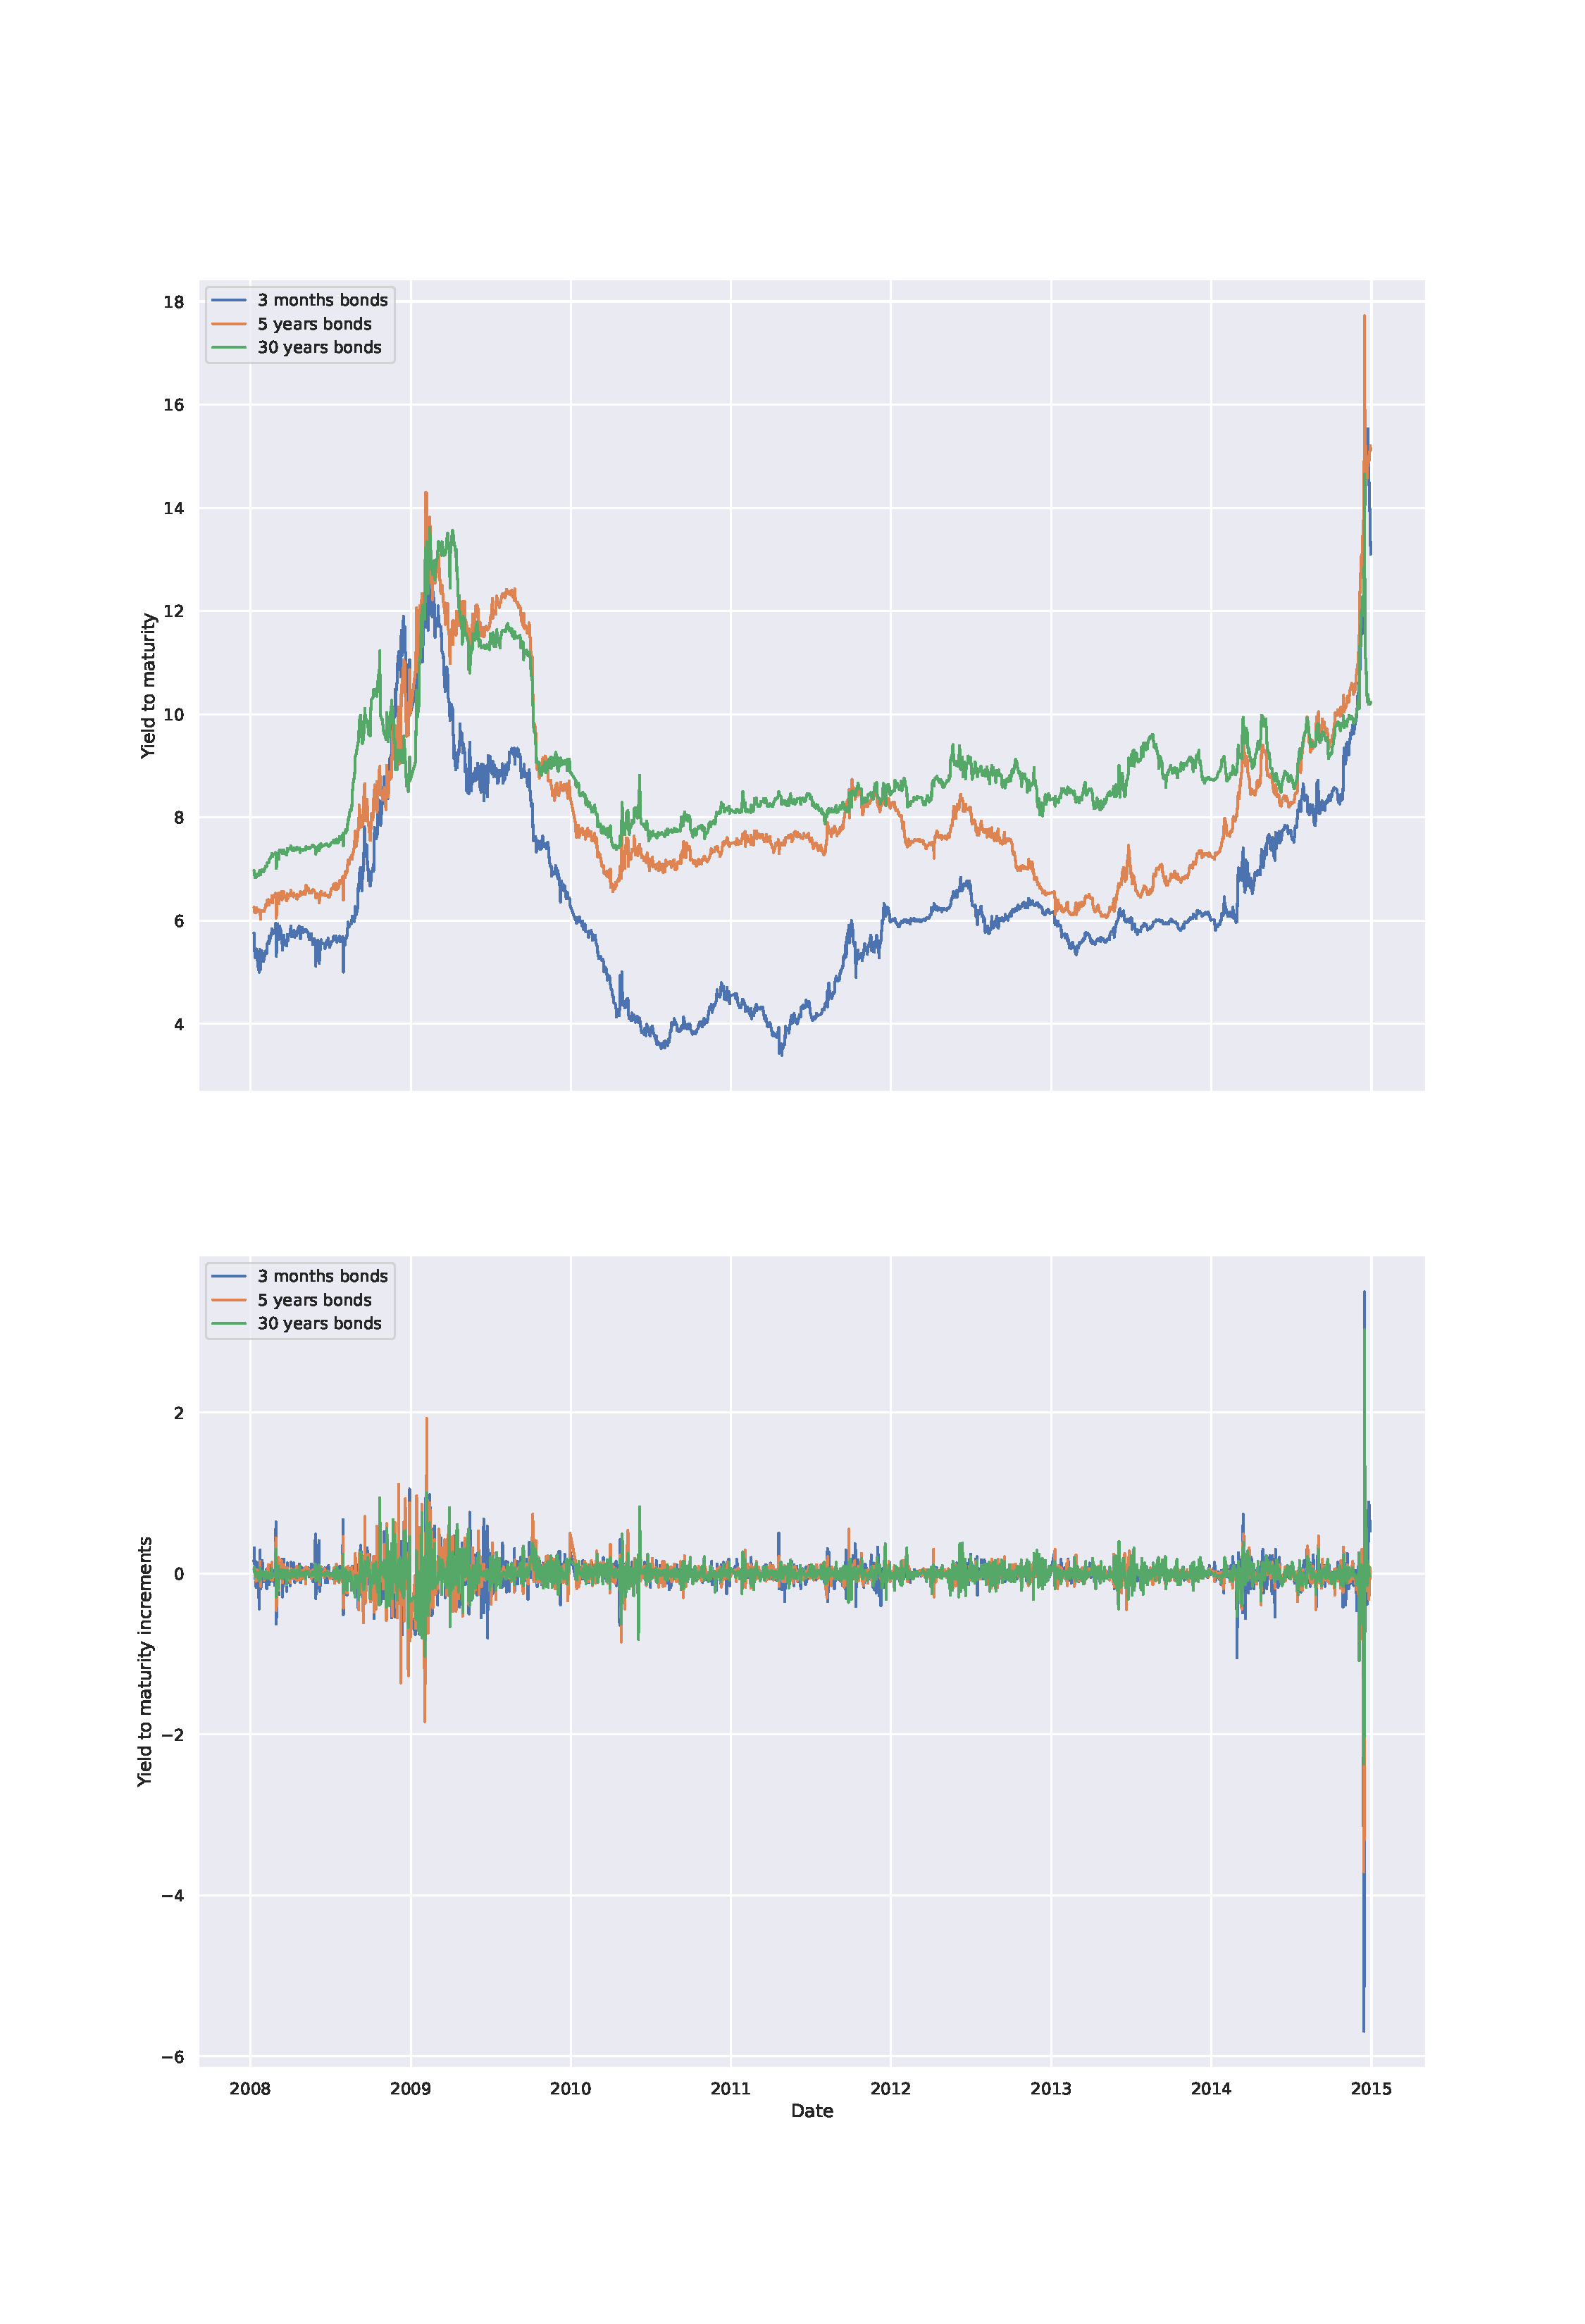
\includegraphics[width=\linewidth]{YTM.pdf}
    \caption{Russian government bond yield to maturity dynamics}
    \label{fig:YTMdynamics}
\end{figure}